\section{Introduction}

% Streaming apps on embedded and mobile -- performance and energy
Streaming sensor processing forms an important workload for embedded
and mobile devices. Supporting these applications requires delivering
reliable performance -- to keep up with the sensor -- with minimal
energy.

% Control systems handle streaming sensor processing well -- formal
% guarantees in the face of dynamics
Control theoretic resource managers have proven ability to deliver
reliable performance with minimal energy.  Examples include mobile
multimedia \cite{grace,grace2,Agilos,flinn2004,xtune,TCST} and
webservers \cite{Horvarth,Verma,LuEtAl-2006a,sha2002queuefeedback}.
In addition to their practical benefits, these control solutions
provide formal guarantees that they will meet the desired performance
despite unpredictable system dynamics; \eg{} changing application
workload or resource availability
\cite{ICSE2014,Hellerstein2004a,KaramanolisEtAl-2005a}.

% Unfortunately, control solutions are brittle, especially challenged
% by diversity of applications and modern heterogeneous processors
While control theory is a general technique, control designs are
problem-specific. Traditional control design directly incorporates
application- and system-specific models that estimate performance and
energy as a function of resource usage.  This requirement -- to
provide specific models at design time -- leads to brittle designs
that only work for limited cases; a problem exacerbated by growing
application diversity and hardware complexity.  For example, modern
embedded and mobile systems rely on heterogeneous processors that
expose a huge range of performance and energy tradeoffs, which vary
from application to application.  \emph{This paper's goal is to
  provide the benefits of control theoretic techniques in a general
  design that provides reliable performance and minimal energy -- even
  for applications we have not encountered before and with minimal
  input from users.}

% Challenges?  
%  We would like to take unseen streaming applications and control them.
%  1) Complexity of system -- non-convex tradeoff spaces
%  2) Cost of learning
%  3) Maintain control theoretic guarantees
Several challenges must be addressed to meet this goal:
\begin{itemize}
\item \textit{System complexity:} Heterogeneous processor designs in
  embedded and mobile systems expose multiple resources that interact
  in complex ways, leading to difficult optimization problems.
\item \textit{Overhead:} We cannot spend more energy solving these
  optimization problems than we would save by knowing the answer.
\item \textit{Guarantees:} We must maintain formal guarantees about
  the controlled system's dynamic behavior.
\end{itemize}


% Therefore we propose CALOREE
To meet these challenges, we propose
\SYSTEM{}\footnote{\textbf{C}ontrol \textbf{A}nd \textbf{L}earning for
  \textbf{O}ptimal \textbf{R}esource \textbf{E}nergy
  \textbf{E}fficiency} to dynamically manage resources for streaming
applications: ensuring their performance needs are met while
minimizing their energy.  While all control-based solutions have a
model-building phase, \SYSTEM{} is unique in that it builds models
online, eliminating the requirement for design-time model
specification.

\SYSTEM{} has two components.  The first is a generalized control
system (GCS) that runs on the embedded or mobile device and
dynamically assigns resources to applications.  The second component
is a hierarchical Bayes\-ian model (HBM) that runs on a remote server.
When the GCS encounters a new application, it samples the
application's performance and energy in a small number of resource
configurations and sends that data to the HBM.  The HBM aggregates
data across devices and applications to estimate the application's
performance and energy tradeoffs.  This estimate is stored in a
performance hash table (PHT) that is sent to the GCS.  Additionally,
the HBM sends the estimated variance so that the GCS tunes its
behavior not just to the estimated model, but also to the error in the
model's output.

% Why CALOREE meets the challenges
\SYSTEM{} addresses the three challenges listed above.  The HBM is
robust to non-convex optimization spaces common to heterogeneous
embedded and mobile processors, addressing the complexity challenge.
The HBM is, however, computationally expensive and requires samples of
several different applications to produce accurate models, so we
offload it to a remote server to address the overhead challenge.
Finally, because the HBM communicates the model's variance and
confidence interval, we derive probabilistic control theoretical
guarantees that the system will converge to the desired performance.

% We implement CALOREE... and our results show...
We test CALOREE controlling streaming applications on heterogeneous ARM
big.LITTLE devices, with the HBM implemented on an x86 server.  As
\SYSTEM{} combines learning and control we evaluate it against
individual state-of-the-art learning and control systems.  We consider
both \emph{single-app} environments, where the streaming application
runs by itself, and \emph{multi-app} environments where other
applications unpredictably enter the system and compete for resources.
We find that \SYSTEM{} achieves the:
\begin{itemize}
\item \textit{Most reliable performance:} 
  \begin{itemize} 
  \item In the \emph{single-app} case, all methods achieve average
    performance close to the requirement.  \SYSTEM{}'s worst case
    performance is within 8\% of the target, while prior techniques
    achieve worst case performance 28\% to 81\% lower than the
    requirement.
  \item In the \emph{multi-app} case, prior learning approaches
    average at least 19\% performance error, prior control approaches
    average 7\% error, and \SYSTEM{} achieves just 3\% average error
    -- less than half the next best.  All prior approaches have a
    worst case performance at least 70\% below the target, while
    \SYSTEM{}'s worst case performance is within 22\% of the target.
    \end{itemize}
  \item \textit{Best energy savings:} We compare to an \emph{oracle}
    with a perfect model of the application, system, and future
    events.
    \begin{itemize}
    \item In the \emph{single-app} case, prior learning approaches
      average 14-21\% more energy than the oracle, while the prior
      controller uses 24\% more (the learners save energy by failing
      to meet the performance requirements).  In contrast, CALOREE
      uses only 4\% more despite providing more reliable performance.
      In the worst case, prior approaches can use 75-90\% more energy
      than the oracle, while CALOREE's worst case is only 24\% more
      than the oracle -- more than $3\times$ energy savings.
    \item In the \emph{multi-app} case, prior learning approaches use
      17-22\% more energy than the oracle.  Prior control approaches
      use 34\% more (again learning saves energy by missing
      deadlines).  CALOREE, in contrast, consumes only 8.5\% more
      energy than the oracle without the oracle's {\em a priori}
      knowledge.
    \end{itemize}
\end{itemize}

% Contributions, but I decided against bulleted llist for thsi paper
In summary, control theoretic approaches are well suited to manage
resources in dynamic environments and machine learning techniques can
produce accurate models of complex processors.  \emph{To the best of
  our knowledge, this is the first work to propose combining the two
  at runtime to control resource usage for a streaming application
  with no prior knowledge.}  Describing the interfaces and design
choices that make this combination work is the paper's primary
contribution.  Additional contributions include formal analysis
showing how to incorporate learned variance into the control theoretic
guarantees and the empirical evaluation showing the combined control
and learning system outperforms individual, state-of-the-art control
or learning solutions.

%%Old intro from ASPLOS 17
\PUNT{
Mobile systems have clear requirements for user satisfaction: they
must meet performance goals necessary for interacting with sensors and
human users while simultaneously conserving energy to maximize battery
life.  To address these conflicting requirements, mobile processors
have become increasingly diverse, exposing heterogeneous resources
that must be managed by software. Meeting performance requirements is
further complicated by the dynamic nature of these systems:
application resource demands can vary widely as a function of input,
application phase, and multiple applications may compete for
resources.

Meeting performance requirements with minimal energy on mobile systems
poses two challenges: \emph{complexity} and \emph{dynamics}.  Machine
learning approaches can handle the complex performance/power tradeoff
spaces that arise on heterogeneous mobile systems
\cite{reddiHPCA2013,dubach2010,Bitirgen2008,Ipek,Koala,LEO,Flicker,Ponamarev},
but they have no established mechanisms for reacting to environmental
fluctuations.  \PUNT{Such approaches can learn complex models,
  identifying and avoiding local extreme that lead to inefficient
  resource usage.}  Control theoretic techniques explicitly address
system and resource dynamics
\cite{Hellerstein2004a,Chen2011,PTRADE,POET,ControlWare,Agilos,grace2},
but rely on linear models that do not capture the diversity of modern
hardware.  \PUNT{Control techniques provide a formal basis for
  reasoning about dynamics and are robust to application, input, and
  workload fluctuations. These approaches have complementary strengths
  and weaknesses.  Learning handle complexity but have no established
  mechanism for managing system dynamics.  Control approaches handle
  dynamics but rely on linear models that do not capture the diversity
  of modern hardware. } Independently, neither control nor learning
meet the challenges of modern mobile resource management.

\begin{figure}
%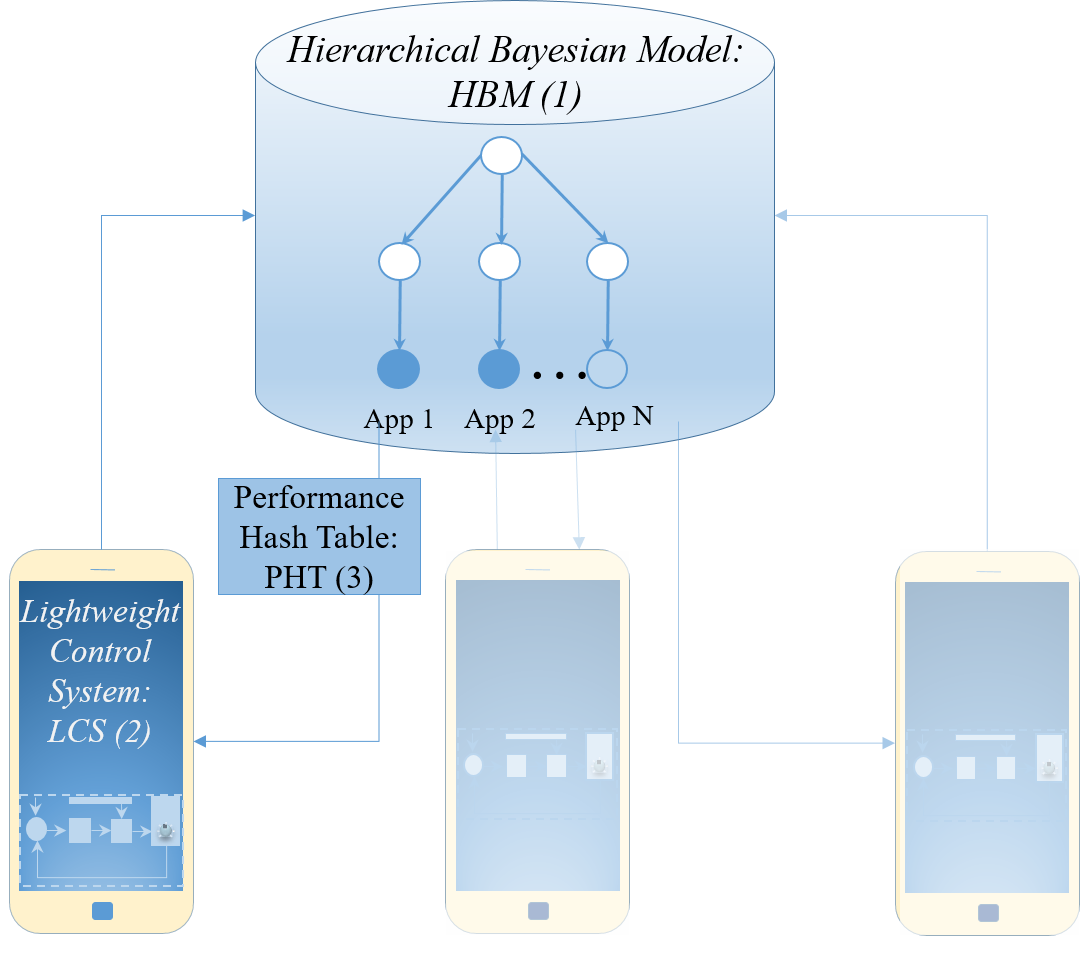
\includegraphics[width=\columnwidth]{figures/Mobile2.png}
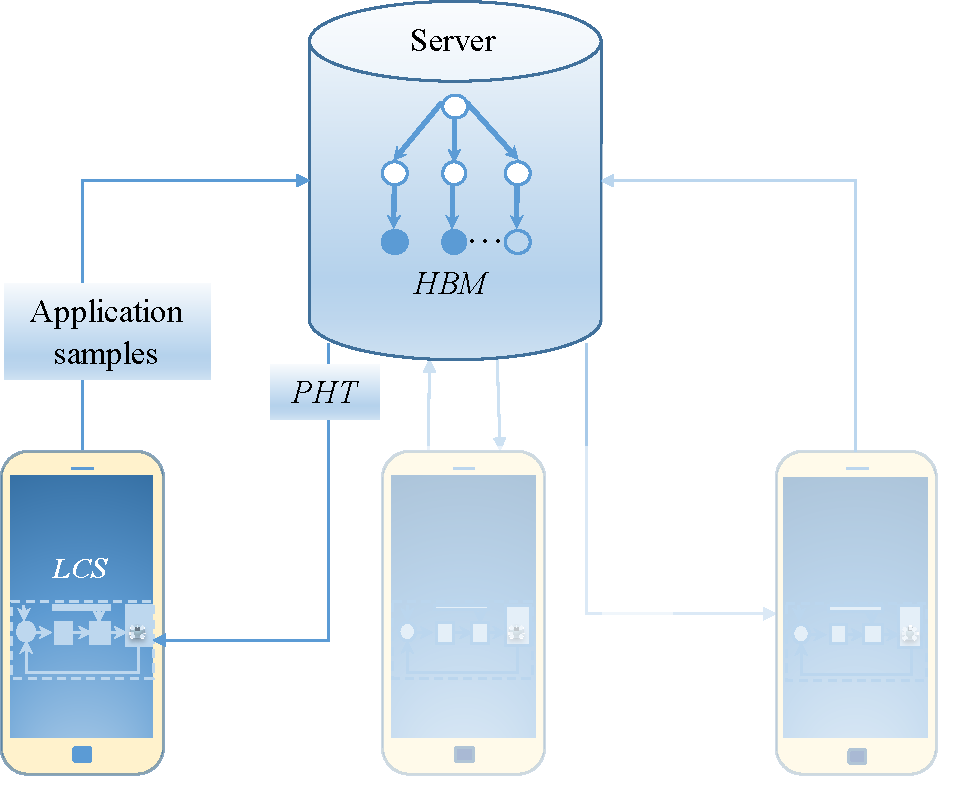
\includegraphics[width=\columnwidth]{figures/mobile-leo-poet2.pdf}
\caption{\SYSTEM{} overview: Mobile devices communicate with a server
  running a hierarchical Bayesian model (HBM) to learn
  performance/power tradeoffs.  The learned model is stored in a
  Performance Hash Table (PHT) and sent to a lightweight control
  system (LCS), which tunes the device's resource usage to meet
  performance goals with minimal energy. }
  \label{fig:overview}
\end{figure}
We therefore propose \SYSTEM{}\footnote{\textbf{C}ontrol \textbf{A}nd
  \textbf{L}earning for \textbf{O}ptimal \textbf{R}esource
  \textbf{E}nergy \textbf{E}fficiency}, a combination of learning and
control consisting of the three components shown in
\figref{fig:overview}: (1) a hierarchical Bayesian model (HBM) that
learns application-specific relationships between performance/power
and resource usage, (2) a lightweight control system (LCS) that
dynamically tunes resource usage to meet performance requirements with
minimal energy, and (3) a performance hash table (PHT), which is the
interface between learning and control.

\PUNT{
\SYSTEM{}'s design has two unique features:
\begin{itemize}
\item \textit{Remote Learning:} Sophisticated learning techniques
  produce accurate models of complicated systems but they are
  computationally expensive.  \SYSTEM{} mitigates this expense by
  running the learner on a remote server. This approach not only
  addresses overhead, it allows the learner to aggregate data from
  multiple devices, improving learning accuracy.
\item \textit{Fast Control:} The controller must not significantly
  impact performance or energy on the mobile device.  Yet, the
  controller must solve a constrained optimization problem to meet the
  performance goal with minimal energy.  To overcome this difficulty,
  \SYSTEM{}'s remote learner constructs a PHT for each application.
  While building the PHT is expensive, it allows the LCS to solve the
  constrained optimization problem in constant ($O(1)$) time.
\end{itemize}
}

\SYSTEM{}'s design has two unique features: \textit{Remote Learning}
and \textit{Fast Control}. First, sophisticated learning techniques
produce accurate models of complicated systems but they are
computationally expensive.  \SYSTEM{} mitigates this expense by
running the learner on a remote server. This approach not only
addresses overhead, it allows the learner to aggregate data from
multiple devices, improving learning accuracy. Second, the controller
must not significantly impact performance or energy on the mobile
device.  Yet, the controller must solve a constrained optimization
problem to meet the performance goal with minimal energy.  To overcome
this difficulty, \SYSTEM{}'s remote learner constructs a PHT for each
application.  While building the PHT is expensive, it allows the LCS
to solve the constrained optimization problem in constant ($O(1)$)
time.

\PUNT{ \SYSTEM{} overcomes three difficulties of combining learning
  and control:
\begin{itemize}
\item \textit{Model differences:} The learner produces non-linear
  models of discrete resources, while the control system is based on
  continuous, linear models.  \SYSTEM{} addresses this challenges by
  scheduling resources in time to map a continuous control into
  discrete resource configurations.
\item \textit{Learning overhead:} Sophisticated learning techniques
  produce accurate models of complicated systems but they are
  computationally expensive.  \SYSTEM{} overcomes this difficulty by
  running the learner on a remote server. This approach not only
  addresses overhead, it allows the learner to aggregate data from
  multiple devices, improving learning accuracy.
\item \textit{Control overhead:} The controller must not significantly
  impact performance or energy on the local device.  Therefore,
  \SYSTEM{} stores the learned models in the PHT, which allows it to
  schedule resources in constant ($O(1)$) time.  
\end{itemize}
The PHT is \SYSTEM{}'s key enabler.  It serves as the interface
between the HBM and LCS, allows the learner to be executed remotely,
and enables fast scheduling on the local device.  } \PUNT{ The main
challenge in combining a learning system with a control system is that
the learner produces non-linear models of resources (\eg cores and
clock speeds) which are discrete, while the control system is based on
continuous linear models.  \SYSTEM{} bridges this gap by scheduling
resources in time to meet a performance requirement with minimal
energy.

The second challenge is that our learner (HBM) produces accurate
models of power and performance, but like many sophisticated machine
learning based models it is computationally expensive, so in \SYSTEM{}
the HBM runs on a remote server.  Moreover, as it is remote, it is
also capable of aggregating data from multiple devices, which makes
learner more powerful. The controller (LCS) runs on individual mobile
devices and receives models from the HBM.

Thirdly, for great user satisfaction, we would like this system to be fast. Hence, we propose that  these models are stored in the PHT, a data structure that allows the LCS to determine energy minimal resource schedules in constant time. The PHT is \SYSTEM{}'s key enabler.  While learning and control
systems exist, their combination requires an appropriate interface.
 %The PHT stores the learned models in such a way that this optimization problem can be solved in constant time, making it appropriate for use on a mobile device.   
While only tested with \SYSTEM{} we believe the PHT is general enough
to be used by different learning and control systems, or even to solve
different optimization problems.  }


% While control and learning frameworks exist, the key to combining
% them is creating an interface between the learning and control
% systems.  Specifically, learning frameworks for resource management
% map configurations (\eg{} resource allocations) into estimated
% performance and power.  These mappings are discrete and non-linear,
% capturing the behavior of the underlying system.  Controllers, in
% contrast, work with continuous linear models.  Therefore, our
% proposed combination of learning and control requires an interface
% to convert the discrete non-linear learned models into continuous
% linear models.  We address this challenge by forming the lower
% convex hull of points on the learned power/performance tradeoff
% space.  Interpolating between these points gives us a piecewise
% linear function that is appropriate for control models, yet still
% captures the significant behavior of the underlying system.  This
% interface allows us to combine the approaches studied in this paper,
% and we believe it is sufficiently general to apply to other
% combinations of learning and control as well.
\PUNT{ We test \SYSTEM{} on ARM big.LITTLE platforms with 20 different
  benchmarks to evaluate the HBM's ability to learn application
  specific models and the LCS's ability to deliver performance
  efficiently.  We compare to published learning and control methods
  in a variety of settings.  While many applications have inherent
  dynamics (\ie{}{} different processing phases), we explicitly test
  the ability to adapt to the unknown by running each application with
  other, random applications.}



We run HBM on an x86 server and the LCS on ARM big.LITTLE devices and
evaluate across 20 parallel benchmarks that exhibit a variety of power
nd performance trade-off behaviors.  We find that \SYSTEM{} delivers:
\begin{itemize}
\item \textbf{Reliable Performance: } \SYSTEM{} achieves an average
  error of 2\%, compared to 4.5-5.4\% for existing learning methods
  and 4.7\% for existing control approaches.
\item \textbf{Lower Average Energy:} \SYSTEM{} achieves an average
  energy consumption of only 7\% over optimal, compared to 25-52\% for
  existing learning methods and 26\% for existing control approaches.
\item \textbf{Better Worst Case Behavior:} \SYSTEM{}'s worst observed
  error across all applications and targets is 9\%, compared to
  19-73\% for prior learning methods and 25\% for existing control
  methods.  The worst observed energy for \SYSTEM{} is 1.82$\times$
  greater than optimal, while it is 4-12$\times$ greater for learning
  and 2.9 $\times$ greater for control.
\item \textbf{Adaptability to Dynamics:} We test \SYSTEM{}'s ability
  to deal with changing environments by introducing resource
  contention with other processes.  In a dynamically fluctuating
  environment, \SYSTEM{}'s worst performance error is 30\%, as
  compared to 71-84\% for prior learning approaches and 35\% for prior
  control approaches.
\end{itemize}

In summary, this paper makes the following contributions:
\begin{itemize}
\item Proposes \SYSTEM{}, a combination of a hierarchical Bayesian
  model with a lightweight control system, which addresses the twin
  challenges of \emph{complexity} and \emph{dynamics} to meet
  application performance goals with minimal energy on heterogeneous
  mobile systems.
\item An interface for combining learned models of discrete resource
  usage with continuous control models of resource dynamics that
  allows the lightweight controller to run in constant time.
\item Demonstrates that \SYSTEM{} achieves both smaller error and
  higher energy savings compared to independent learning and control
  techniques.
\end{itemize}
}